\chapter{Efficiencies}
\label{sec:Efficiencies}

The detection and reconstruction of particle decays is not perfect at all, i.e. not all particles and tracks originating from the \proton\proton interaction are detected and recorded.
This ratio of the recorded signal yields and the total number of decays is referred to as ``efficiencies".
There are several reasons for inefficiencies.
Here are some examples:
\begin{itemize}
    \item Particles escape the geometrical detector acceptance.
    \item A particle traverses a sensor during the dead time of a sensor, i.e. a signal caused by an earlier particle is still processed. 
          In this time, the sensor is not able to process the second signal.
    \item Applying selection requirements for the reduction of backgrounds prevents signal events to pass these requirements as well
    \item ...
\end{itemize}
For the measurement of the number of signal events the exact knowledge / determination of all efficiencies is crucial.
The way how the efficiencies for the \LbToDpmunuX and \LbToLcmunu decays are accounted for the measurement of the relative branching ratio \R is shown in equation (\ref{eq:R}).

For this analysis, the efficiencies are determined using simulated events.
These simulation samples contain information about all generated as well as reconstructed events for which detector effects are accounted for.
The simple way is to divide the number of reconstructed and selected simulated events by the number of generated events. 
This efficiency is hereafter called selection efficiency \effSel.
Nonetheless, the generation of the events is not efficient at all. 
Several requirements are already applied during generation to reduce the computation time of the simulation production.
Above all, the simulation of the detector takes a lot of time.
That is why all generated events are required to be in the \lhcb acceptance.
A further acceleration of the production process can be achieved with additional requirements on the final state particles' (transverse) momenta.
Concerning the \LbToDpmunuX and \LbToLcmunu channel these requirements are different and likewise the efficiencies of the generation process.
Thus, the so-called generator level efficiency \effGen also has to be determined for both channels. 
The total efficiency used for the calculation of \R is the product $\effGen \cdot \effSel$.

Unfortunately, it is known that the simulations do not perfectly describe the data. 
Since the decay \LbToDpmunuX is not well-known the physical properties are not correctly modeled in simulation and thus disagree with data.
Additionally, no theoretical prediction of the \LbToDpmunuX channel is available.
The plots in Figure \ref{fig:reweighting} show a comparison of data (black points) and the simulation (red lines).
A huge disagreement between the (unweighted) simulation and data can be seen, above all in the \MDp and \MDmu distributions.
In order to adjust the decay kinematics the simulated events hence have to be reweighted.
This leads to a more proper estimate of the efficiency.
Several reweigthing steps are applied and will be described in the following.
The effect of the reweighting is also shown in Figure \ref{fig:reweighting}.
A discussion on it follows.
\begin{figure}[hptb]
	\centering
	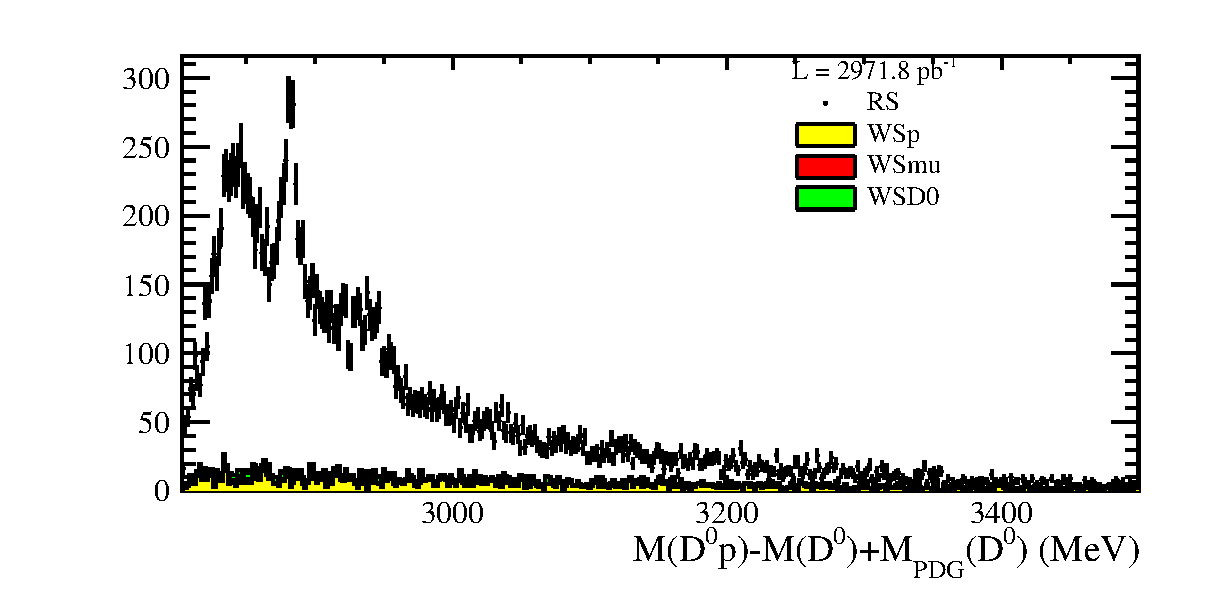
\includegraphics[width=0.49\textwidth]{LbToD0p/comparisons/3D/mD0p_mD0mu_mD0pmu/20Bins/20.0MaxWeight/Bh_DELTA_MASS}
	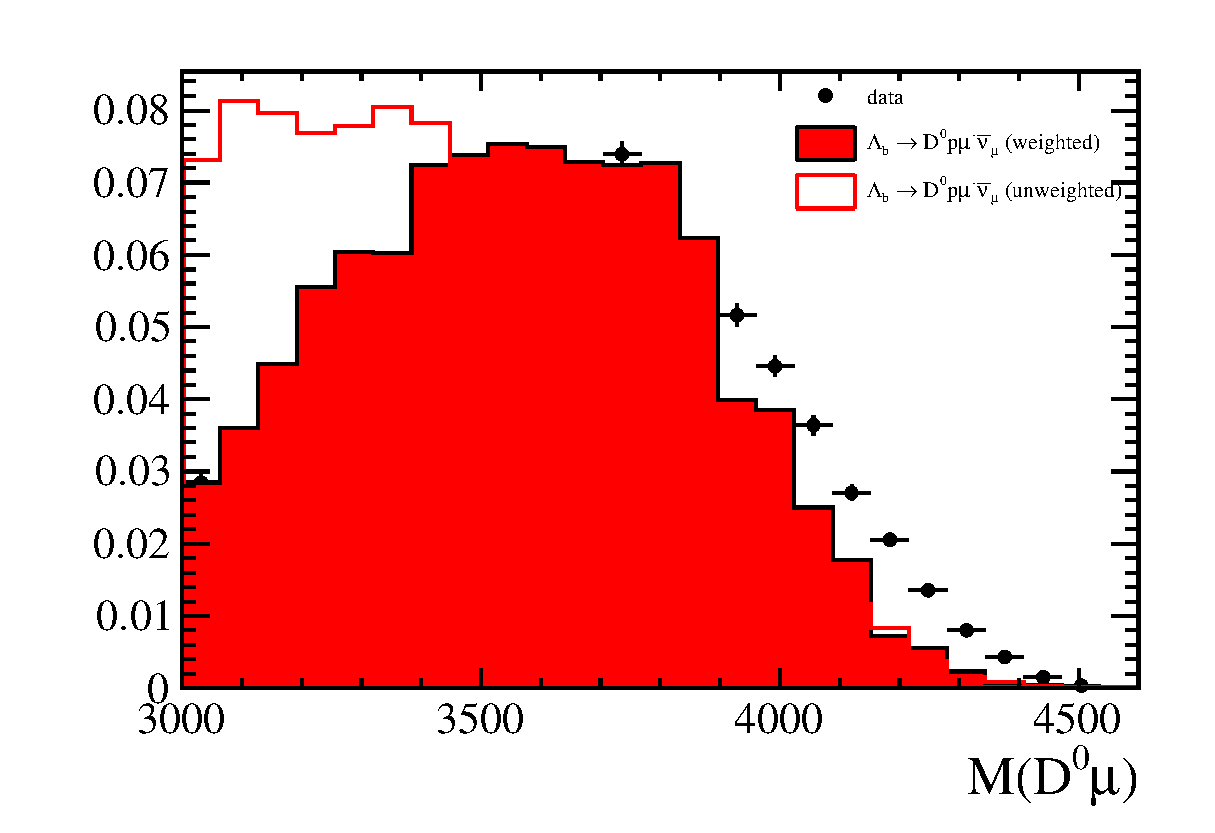
\includegraphics[width=0.49\textwidth]{LbToD0p/comparisons/3D/mD0p_mD0mu_mD0pmu/20Bins/20.0MaxWeight/B_M}
	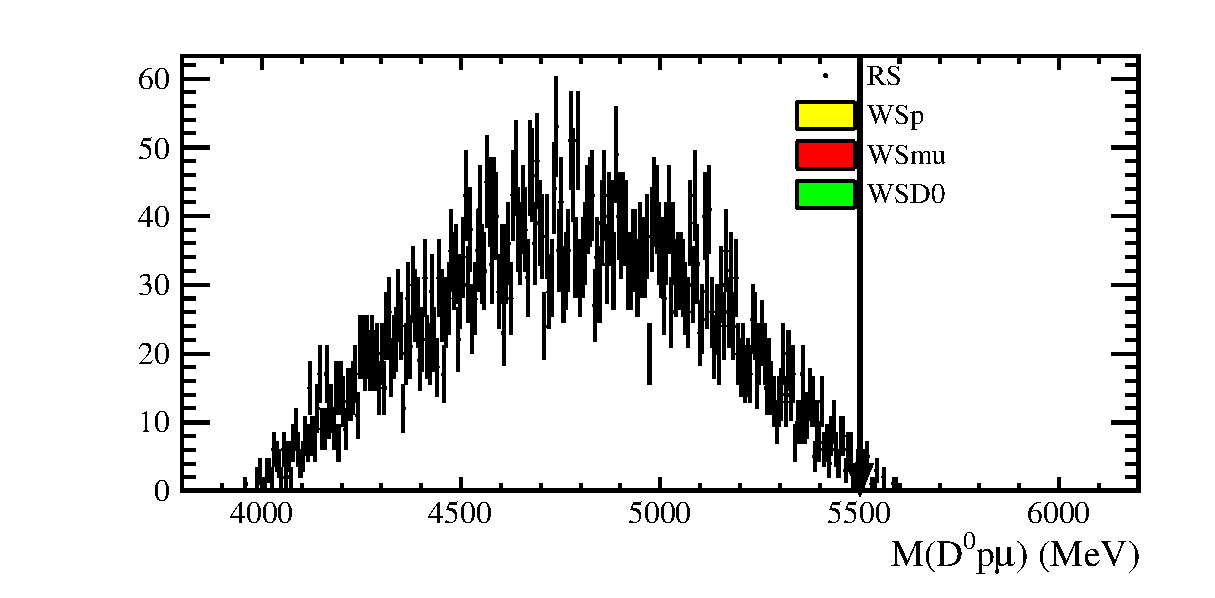
\includegraphics[width=0.49\textwidth]{LbToD0p/comparisons/3D/mD0p_mD0mu_mD0pmu/20Bins/20.0MaxWeight/Bh_M}
	\caption{Comparison of data (black points) and simulation for the \LbToDpmunuX channel before (red line) and after (red shaded area) threedimensional reweighting as described in the text (see sec. \ref{sec:Reweight_D0p}).}
	\label{fig:reweighting}
\end{figure}

\section{Kinematic reweighting of the simulated \LbToDpmunuX and \LbToLcmunu decays}
The production of \Lb baryons depends strongly on their transverse momentum as Figure \ref{fig:LbPTrew} (left) from reference \cite{Lb_production_kinematic} shows. 
This dependence is not well emulated in the simulation and thus has to be corrected. 
This was already done in the semileptonic \lhcb-measurement of $|\Vub|$ in ref. \cite{SL_Vub} using the decay \decay{\Lb}{\jpsi\Dz\proton}. 
To calculate the weights data and simulation of this hadronic \Lb decay channel was compared as shown in Figure \ref{fig:LbPTrew} (right). 
In this analysis, the applied weights are determined from the same channel with the help of the distributions in Figure \ref{fig:LbPTrew} (right).
The reweighting is applied in both, \LbToDpmunuX and \LbToLcmunu, channels according to the true \Lb transverse momentum \pt, i.e. the actual generated transverse momentum.
\begin{figure}[hptb]
	\centering
	\includegraphics[width=0.49\textwidth]{Lb_production_pt_dependence}
	\includegraphics[width=0.49\textwidth]{Lb_pt_comparison_weights}
	\caption{Left: Ratio of \Lb to \Bd production as a function of \pt. Figure taken from \cite{Lb_production_kinematic}.  Right: Transverse \Lb momentum for \decay{\Lb}{\jpsi\Dz\proton} decays in data and simulation. Figure taken from the documentation belonging to \cite{SL_Vub}.}
	\label{fig:LbPTrew}
\end{figure}


\section{Reweighting of the simulated \LbToDpmunuX decays}
\label{sec:Reweight_D0p}
It has already been mentioned that the underlying physics in the \LbToDpmunuX simulation is not correctly modeled.
Since there are not any theoretical predictions for that channel, the reweighting of the simulation has to be done directly on data.
To come as close to data as possible, a three-dimensional reweighting in the variables, M(\Dz\proton), M(\Dz\mun), M(\Dz\proton\mun) has been chosen. 
This choice is not trivial and above all not obvious, but there are several reasons for it:
\begin{enumerate}
    \item The simulation shows large differences compared to the data distribution in these variables.
    \item These variables are already available at generator level, i.e. before detector effects are simulated. 
          To calculate the selection efficiency the simulation has to be reweighted at generator stage as well.
    \item There are not any selection requirements on these variables. 
          Otherwise, no weights could be assigned to events, not fulfilling the requirements.
          \footnote{There exists a selection requirement on M(\Dz\proton\mun) in this analysis to eliminate \decay{\Lb}{\Dz\proton\pim} background, but less than 0.5\% of all events have their generated mass above this value. 
                    Thus, its impact on the efficiency can be neglected.}.
\end{enumerate}
The reweighting and the calculation of the efficiencies is performed with the following steps:
\begin{enumerate}
    \item \textbf{Determination of the weights} \\
          There are two normalised three-dimensional histograms drawn for both, generated events and events after reconstruction, applying selection cuts and the kinematic reweighting. 
          The dimensions of these histograms are the three mass variables mentioned above.
          The histogram containing the weights is now calculated by dividing the histogram with the selected events through the histogram containing the generated events.
    \item \textbf{Assigning weights to the events} \\
          Now, this weight histogram is used to assign a weight to each selected and generated event.
          In the following, the weights are denoted with \weight{sel}{} respectively \weight{gen}{}.
          To get the correct bin in the weight histogram the generated masses \Mtrue{\Dz\proton}, \Mtrue{\Dz\mun} and \Mtrue{\Dz\proton\mun} are used.
    \item \textbf{Calculation of the efficiency} \\
          The efficiency is calculated with
          \begin{align}
              \epsilon = \frac{\sum\limits_{i=1}^{N_\text{sel}} \weight{sel}{i}}{\sum\limits_{i=1}^{N_\text{gen}} \weight{gen}{i}}, \label{eq:effrew}
          \end{align}
          where $N_\text{sel}$ and $N_\text{gen}$ denote the number of selected respectively generated events.
          To account for the loss of statistical power due to reweighting, both the numerator and denominator in equation (\ref{eq:effrew}) are multiplied by the renormalisation factor $\sum \weight{gen}{} / \sum (\weight{gen}{})^2$. 
          This does not affect the central value of $\epsilon$ but influences the statistical error, which is calculated using binomial statistics.
\end{enumerate}
It becomes clear, that with this procedure one must not apply selection requirements on the weighting variables, since otherwise the weights outside the cut region are zero. 
Hence it would not be clear how to reweight the generated events not fulfilling the selection requirements. 
The distribution of the masses after reweighting are shown in Figure \ref{fig:reweighting}.
A decided improvement of the data description can be figured out.
Some discrepancies can be seen at higher \Dz\mun and \Dz\proton\mun masses.
They arise due to empty bins in either data or simulation.
The last two bins in \MDmu in Figure \ref{fig:reweighting} serve as an good example.
No simulated events exist here, though there is still data.
Nonetheless, these events are weighted with zero, resulting in slight discrepancies.
Many more comparisons between data and simulation before and after reweighting can be found in the appendix \ref{app:Reweight_D0p} in figure \ref{fig:reweight_D0p_app}.

Concerning the channel \LbToLcmunu no further reweighting is applied since the agreement in the comparison between data and simulation seems to be sufficient.
Several comparison plots for this channel can be found in figure \ref{fig:reweight_Lc_app} in \ref{app:Reweight_Lc}.

With this framework, the efficiencies are calculated at different stages of the simulation process.
For each, \LbToDpmunuX and \LbToLcmunu decays, there exists two simulations.
First of all, events are generated without any requirements.
Since the simulation of the detector takes a lot of time, first requirements on the \lhcb detector geometry are applied.
Thus, the so-called generator level simulation sample contains these generated events and the events passing the geometry requirements.
The effciency corresponding to these requirements is hereafter called generator level efficiency \effGen\footnote{This naming convention must not be mixed up with naming of the weights \weight{sel}{} and \weight{gen}{}}.
The second simulation sample contains fully simulated events having passed the requirements in the generator level simulation.
In this sample there is again a set of generated events and another set of selection events after passing the whole reconstruction process described in Chapter \ref{Selection}.
In the following, the effenciency corresponding to this second sample is called selection efficiency \effSel.

\section{Generator level efficiencies}
As a reminder, generator level efficiencies arise due to the fact, that one demands the generated events to be in the \lhcb acceptance and apply some (loose) requirements on the kinematics to accelerate the simulation process.
The generator level samples are reweighted as described above: the \LbToLcmunu sample with the kinematic \pt(\Lb) reweighting and the \LbToDpmunu sample with both reweightings.
For signal and normalization channel the following generator level efficiencies are obtained:
\begin{align*}
    \effGenLc &= \effGenLcval \pm \effGenLcerr, \\
    \effGenDp &= \effGenDpval \pm \effGenDperr.
\end{align*}

\section{Reconstruction and selection efficiencies}
The reconstruction and selection efficiencies are calculated analogously.
The same reweighting procedure on the different samples is performed.
The results for signal and normalization channel are:
\begin{align*}
    \effSelLc &= \num[scientific-notation=true]{\effSelLcval \pm \effSelLcerr}, \\
    \effSelDp &= \num[scientific-notation=true]{\effSelDpval \pm \effSelDperr}.
\end{align*}

\section{Total efficiencies}
To summarise the values above the total efficiencies for the channels are:
\begin{align*}
    \effDp &= \effGenDp \cdot \effSelDp = \num[scientific-notation=true]{\effDpval \pm \effDperr}, \\
    \effLc &= \effGenLc \cdot \effSelLc = \num[scientific-notation=true]{\effLcval \pm \effLcerr}.
\end{align*}
This results in an efficiency ratio of
\begin{align*}
    \frac{\effLc}{\effDp} = \effRatioval \pm \effRatioerr,
\end{align*}
which is later used when determining the relative branching ratio \R.
